\documentclass{report}
\usepackage[T1]{fontenc}
\usepackage[margin=0.75in]{geometry}
\usepackage[bottom]{footmisc}
\usepackage{float}
\usepackage{placeins}
\usepackage{booktabs}
\usepackage{xcolor}
\usepackage{listings}
\usepackage{url}
\usepackage{graphicx}
\usepackage{verbatim}
\usepackage{ftnxtra}
\usepackage{fnpos}
\usepackage{caption}
\usepackage{subcaption}
\usepackage{amsmath}

\usepackage{hyperref}
\hypersetup{
    colorlinks,
    citecolor=blue,
    filecolor=blue,
    linkcolor=blue,
    urlcolor=blue
}

\setlength{\parindent}{0cm}
\setlength{\parskip}{10px plus3px minus 3px}

\title{Date matching using Face Recognition}
\author{Davide Berdin, Tobias Famulla \\
  \texttt{ \{davide.berdin.0110\},\{tobias.famulla.7003\}@student.uu.se} \\
  \\ Machine Learning Project
  \\ Department of Information Technology}

\begin{document}

\maketitle
\newpage

\tableofcontents{}

\begin{abstract}
In this project we present a Date Matching application using Face Recognition. For each user that took part of our experiment we created different models using different features extractions and classifiers as well. Our analysis shows a comparison between four different algorithms for human face features extraction, such as Eigenfaces, Fisherfaces, Local Binary Patterns Histograms and Identity. Moreover, for each feature extraction algorithm we applied the K-Nearest Neighbour classifier with Euclidean and Chi-square distances.
\end{abstract}

%%%%
\chapter{Introduction}
The general idea of our project is based on the question how predictable humans are.
As mentioned in the Artificial Intelligence and Machine Learning courses, artificial intelligence in general is associated with a touch of magic, which is hard to understand by humans.
The same picture is drawn concerning another topic: love and attraction.
Despite some clear research results in biology and psychology humans try to believe that these topics are not rational explainable and not calculable.

We thought it might be an interesting project to bring these two topics together.
Although we assume that attraction is a quite complicated field and can not be solved in a small project, a very successful app, Tinder, breaks the properties of attraction down to a simple binary question: Like or Don't-Like based just on the look of the persons.

The condensed question for our project concerning the further will be whether human taste concerning the face of a person is predictable, and how is it predictable.
As we found out, we are not the first people asking and an application called "Tinderbox"\cite{tinderbox}, which does face recognition to automatically rate persons on Tinder, exist.
To focus more on the face recognition and machine learning aspect of this question, we gathered data concerning pictures and tested different algorithm for the purpose to select people the user might like.

In the following we describe how we gathered data to test on, which algorithms we looked at and how we tested the data.

\chapter{Data Gathering}
\label{ch:datagathering}
To test Face Recognition and Machine Learning algorithms we needed data.
To get these data we decided to program a webapplication, which reimplements the functionality of Tinder.
For this app we used the framework Flask\cite{flask} in connection with SQLAlchemy\cite{sqlalchemy}, SQLite\cite{sqlite} and WTForms\cite{wtforms}.
Testers created a user, got pictures of a person shown and decided whether they liked the person.
After that the next person appeared.
We saved the data to a database and to split these data in training and test-sets to challange the algorithms.

Because we needed a high amount of profile pictures of a certain type (people in age-range which is the preferences of the test-users), we decided to gather these from Tinder directly.
For this we used a public description of the reverse-engineered Tinder-API\cite{tinder-api} and wrote a script to download pictures from people of different cities using our own Facebook-Tokens used by Tinder \footnote{
Because the pictures are freely available to all Tinder-users, we assume that using them in a scientific project should not be problematic.
The web application was just accessable by a small group of users to generate the data for the project.
Due to legal concerns we will not make the picture-set publicly available, but provide a script with the sourcecode of the project.}

After preprocessing the photos (see Chapter \ref{ch:test}) we got around 300 male and the same amount of female people, which had three pictures each to use for face recognition.

The webapp has been used by a pool of 8 testers and got 5 complete datasets including our own, meaning that each user rated all pictures according to their sexual preference.
The uncomplete datasets contained a certain amount of rated persons, but not all people of a gender.

In the following we describe the different algorithms applicable for our problem and later on how we used them.

\chapter{Face Detection and Face Recognition}
\textbf{Face detection} is a system that tries to identify human faces in digital pictures. In general, object detection is used in multiple real-world applications nowadays, such as: localization of objects in images or videos, identification of pedestrians or cars, etc. Although, face detections algorithms focus primarily on the detection of frontal human faces \cite{face-detection-wiki}. In our approach we used \textbf{Haar Feature-based Cascade Classifier}, a famous classifier for object detection (see \ref{sec:haar}).

A \textbf{facial recognition} system is an application for automatically identifying a person from either a picture or a video. One of the ways to do this is by comparing selected facial features from the image and a facial database \cite{face-recognition-wiki}.
Given an image in which the face of a subject is present, a facial recognition algorithm tries to identify human facial features by extracting features from the image itself.
In general, it will analyze the relative position of eyes, nose, mouth, etc. The position is not the only variable involved: in fact, size and shape are taken in consideration for a more accurate analysis. All these features will be then used to search for other images in a dataset that will match the original face.

In general, recognition algorithms can be of two kinds: geometric and statistical. The first approach distinguish features, whereas the second approach converts a picture into values and then compare those values with templates in such a way to eliminate the variance.

General methods such as \textit{Principal Component Analysis} (PCA), \textit{Hidenn Markov Model} (HMM) and \textit{Linear Discriminate Analysis} (LDA) are used in face recognition systems. Commons systems are \textit{Eigenfaces} using PCA (see \ref{sec:eigen}) and \textbf{Fisherfaces} using LDA (see \ref{sec:fisherfaces}).

\section{Haar Feature-based Cascade Classifier for Object Detection}
\label{sec:haar}
The following sections describe the classifier algorithm used to detect specific human face features in an image. \textbf{Haar features} are simple and inexpensive image features based on intensity differences between rectangle-based regions that share similar shapes to "square-shaped" functions \cite{oren1997pedestrian}\cite{papageorgiou2000trainable}\cite{features}.

\subsection{Local invariant feature detectors}
Local feature-based methods are an often used group of object recognition methods\cite{tuytelaars2008local}. Haar features are built on the notion of trying to define a set of data for \textit{processing} as well as for providing invariance to different transformations. In the case of Local invariant features, global features are not considered, instead, local feature detection approaches search for \textbf{anchor} points in the picture where local are defined by differences in either texture or intensity. An anchor point, or insterested point, is the type of shape that the algorithm is looking for and it can be an edge or a corner.
To find these textures or intesity changes, a \textbf{kernel} runs over the image. A kernel is a set of pixels computations of computing the gradient change value (the derivative) within this set. These features can be corners, T-junctions, circles, etc., depending on what kind of detector is used \cite{reinius2013object}\cite{tuytelaars2008local}.

\subsection{Haar classification}
The Haar feature-based cascade classifier has been initially proposed in \cite{viola2001rapid} and improved in \cite{lienhart2002extended}.
In fact, the face detection algorithm seeks for specific Haar features of a human face. When a feature is found, the algorithm sends the face candidate to the next step of detection. Basically, a face candidate is a rectangular section of the initial image named \textbf{sub-window}. According to \cite{heisele2001face}, a sub-window has typically a fixed size of 24x24 pixels. Moreover, the sub-window is often scaled in order to get a set of different size faces \cite{tripathyreal}.

The classifier is called \textbf{cascade} (a degenerate decision tree), because the resultant classifier consists of multiple weak classifiers, called stages, that are applied one after another to a region of interest. They are called weak classifiers because if they are taken singularly they cannot classify an image, instead, if combined with others, they can form a strong classifier.

The detection process starts with the evaluation of the first classifier. If its result is positive then the classifier triggers the evaluation of the second one. Given a positive evaluation of the second classifier, a third one is triggered, and so on. As soon as a negative outcome is given, the sub-window is rejected. The evaluation of each classifier is done by a \textbf{stage comparator} where all the previous stages will be summed up and compared to a stage threshold to determine if the stage should be passed or not. If all the stages are passed, the face candidate is concluded to be a face \cite{tripathyreal}.

\section{Eigenfaces}
\label{sec:eigen}
In computer vision problem, the \textit{eigenfaces} in human face recognition is the name given to a set of \textbf{eigenvectors}. An eigenvector of a linear transformation between vector spaces is a vector where the image is the vector itself moltiplied by a scalar vector, called \textbf{eigenvalue}. This can be written as follow:
\begin{equation}
  A\textbf{v} = \lambda \textbf{v}
\end{equation}
where $\lambda$ is the eigenvalue associated with the eigenvector \textbf{v} and \textbf{A} is the square matrix.
This approach was for the first time used in face classification in \cite{turk1991face}.
Each eigenvector is extracted from the \textbf{covariance matrix}, that is a matrix that represents the variation of each variable respects all the others (including the variable itself). The covariance is the value that represents the variation of two variables together.
In other words, the eigenface is a set of values of linearly uncorrelated variables of a distribution of faces where all the pixels in each image is a vector in N-dimensional space. This leads to reduce the number of dimension by using a smaller set of basis pictures to represent the original images for the training set. To classify faces, the algorithm simply compare the faces representation in the basis set.

To generate the eigenfaces' set, the process called \textit{principal component analysis (PCA)} is used over a large set of images with different faces. When an eigenface is created, the resultant image will appear with some light and dark areas arranged to a specific pattern. Figure \ref{fig:eigenfaces} shows how an image is transformed when the eigenfaces are created. Patterns are selected to be evaluated and scored on different features of a human face. Many patterns are involved in facial recognition: evaluation of the face symmetry, facial hair style, position of the hairline, nose size, and so on.
Due to the nature of the algorithm, the dimension reduction method allows the system to represent many subjects with a small dataset. The sensitivity of the recognition system depends on how large are the reductions applied to the image because when the variation between the image we want to recognize and the examined picture is large, the system starts to fail.

For each subject's face in the dataset, a weight describing the contribution of each eigenface gives to the image, is stored in a structure.
When we need to classify a face, a new set of weights of the candidate image is projected onto the collection of eigenfaces providing a collection of weights representing the examined face. All these weights are then compared with all the weights in the previous set for finding the closest match. A typical method for classification used with eigenfaces is \textit{K-NN (nearest neighbour method)} using \textit{Euclidean Distance} between two vectors where the closest subject is given by the minimum distance \cite{turk1991face}.

\begin{figure}[!htb]
  \centering
  \begin{subfigure}{.5\textwidth}
    \centering
    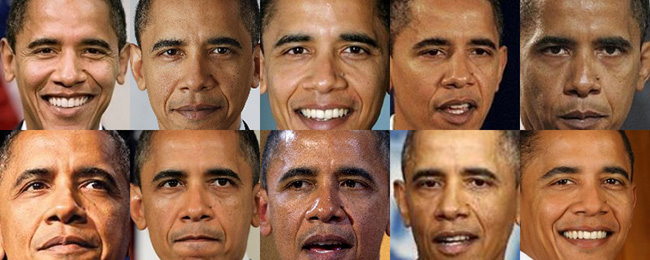
\includegraphics[scale=0.35]{images/obama_normal.png}
    \caption{Training set of pictures}
  \end{subfigure}%
  \begin{subfigure}{.5\textwidth}
    \centering
    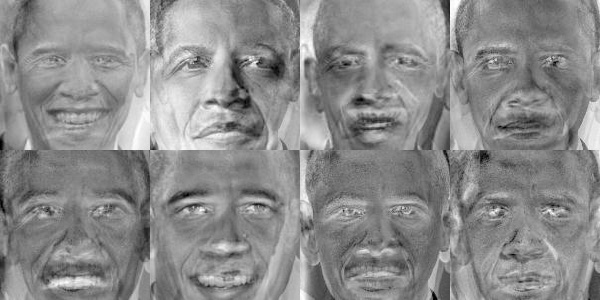
\includegraphics[scale=0.35]{images/obama_eigenface.png}
    \caption{Eigenfaces representation}
  \end{subfigure}
  \caption{Transofrmation from normal pictures to the eigenfaces}
  \label{fig:eigenfaces}
\end{figure}

\newpage

\section{Fisherfaces}
\label{sec:fisherfaces}
The usage of \textit{eigenvectors} is indeed a good way to represent images, because it guarantees that the data variance is kept whilst the algorithm eliminates unnecessary existing correlations between the original features (dimensions) in the sample vectors \cite{fisherfacec-wiki}. When we need to deal with classification instead of representation, eigenfaces may not yield the most desirable results, and since for our project we want the best classification possible the \textbf{Fisherfaces} is introduced. The algorithm uses a techinique called \textit{Linear Discriminant Analysis (LDA)}. When the LDA is used to find the subspace representation of set of pictures, the resulting basis vectors that define this space are known as \textit{Fisherfaces} \cite{fisherfacec-wiki}.
According to \cite{belhumeur1997eigenfaces}, Fisherfaces appears to be the best at extrapolating and interpolating over variation in lighting. Figure \ref{fig:fisherafaces} shows the face features highlights of the Fisherfaces algorithm.

\begin{figure}[!htb]
  \centering
  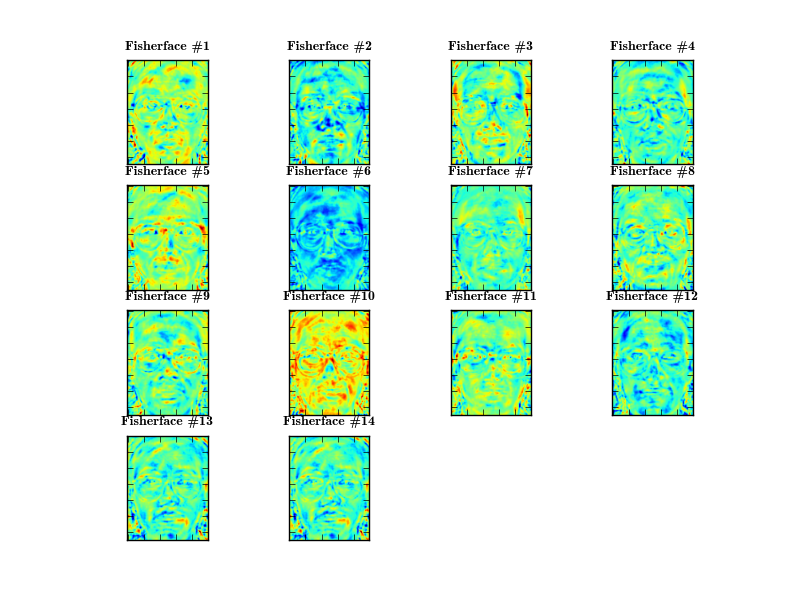
\includegraphics[scale=0.7]{images/fisherfaces.png}
  \caption{Fisherfaces representation of the Yale Facedatabase A}
  \label{fig:fisherafaces}
\end{figure}

\section{Local Binary Patterns Histograms}
Local binary patterns (LBP) method is a texture operator that assigns a label to each pixel of an image by converting an image from greyscale to binary with a non-linear operation. The conversion is called \textbf{thresholding} meaning that if a pixel's value is lower then a specific value (threshold) the value 0 is assigned, 1 otherwise \cite{thresholding}. LBP uses a \textbf{neighbourhood thresholding} which means that a section of 3x3 pixels for each frame in the picture is taken in consideration when assigning a label. The result is then transformed into a binary number. Figure \ref{fig:lbp-comp} shows the transformation process.

A more sofisticated usage of the neighbourhood section has been introduced later in \cite{ojala2002multiresolution} using a circular neighborhood and bilinearly interpolating values at non-integer pixel coordinates \cite{lbp-scholar}.
One the most important feature of LBP is its robustness to \textit{monotonic gray-scale} changes due to the illumination variations of pictures.

\begin{figure}[!htb]
  \centering
  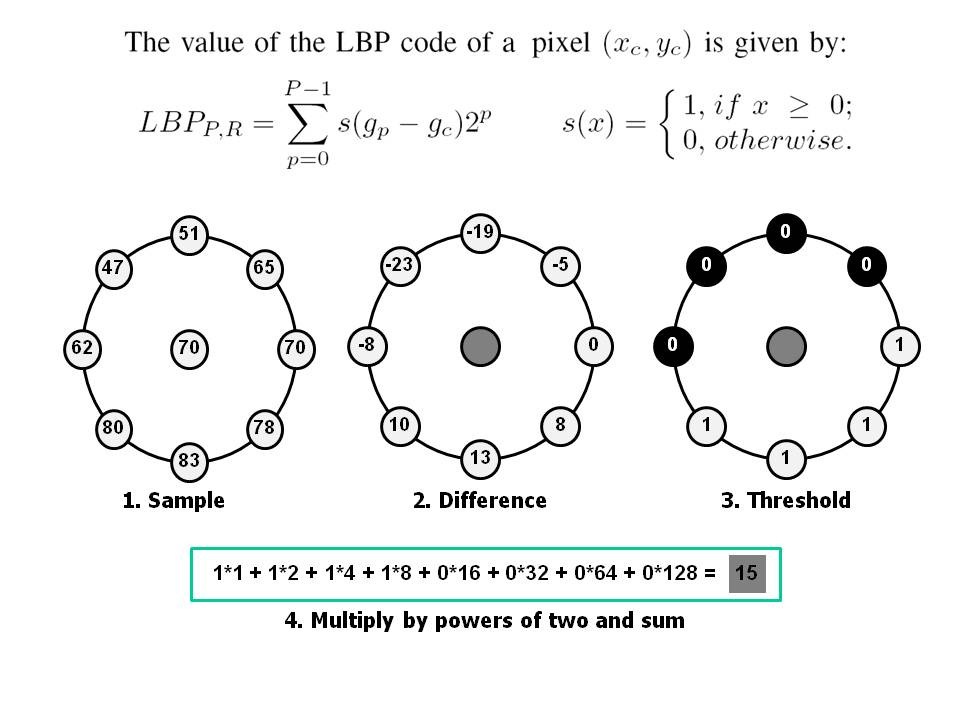
\includegraphics[scale=0.5]{images/lbp-computation.png}
  \caption{An example of LBP computation\cite{lbp-scholar}}
  \label{fig:lbp-comp}
\end{figure}

The LBP approach for classifying a texture is made by collecting the occurrences into a histogram. The classification itself is then done by computing the similarity among all the histograms.
Although, for facial image recognition the approach loses spatial information and therefore the algorithm should also take the location of the texture into account.
An effective method to accomplish this task is using the LBP texture \textit{descriptors} to construct quite a variety of \textit{local descriptor} of the face.
After that these local descriptors can be combined in a unique descriptor called \textit{global descriptor}. The usage of these local descriptors has been found to be more robust against the variation of poses of the face and illumination compared to holistic appreaches like eigenfaces and fisherfaces \cite{parmar2014face}.

The basic methodology for Local Binary Patterns in face recognition was first introduced in \cite{ahonen2006face} and the procedure is described as follows:

\begin{itemize}
  \item The picture with the face is divided into local regions (neighbourhood approach)
  \item The LBP texture descriptors are then extracted from the each region
  \item The descriptors are then concatenated to build the global descriptor
\end{itemize}

Figure \ref{fig:lbp} shows the procedure described above. The resultant histogram contains a description of the face split on three levels of locality: the labels contain the information related to the patterns on fragment level, labels from a small region are then summed up to produce information on a regional level and these regions are then combined to construct the global descriptor.

\begin{figure}[htb]
  \centering
  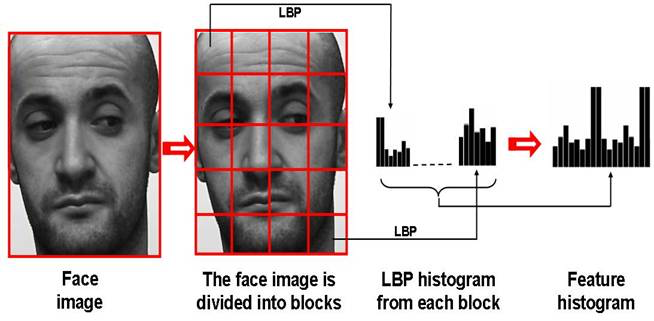
\includegraphics[scale=1]{images/lbp.png}
  \caption{Face description with local binary patterns \cite{lbp-scholar}}
  \label{fig:lbp}
\end{figure}

\chapter{Model Prediction}
To help the user to auto-select a suitable mate, we introduced a \textit{model prediction system} based on the taste of the user. In fact, during the \textit{training phase}, the user selects which are the persons he/she would more likely go out with and which not. With this we create a dataset that we will use for our prediction system.

A simple definition of model prediction system is the ability of predicting the future through the usage of one or more classifiers. The classifier will try to determine the probability of a set of data belonging to another set. Applied to our case, when the training phase is completed, a testing phase will determine the \textit{accuracy} of our model.

\section{Classification models}
\label{sec:models}
Facerec provides two classifiers: \textit{K-Nearest Neighbor} and \textit{Support Vector Machines}. Despite the limited amount of solutions, these classifiers are both suitable for our project.

\textbf{K-Nearest Neighbor} is a \textbf{non-parametric} method. It means that it makes no assumptions about the probability distributions of the variables being assessed for either classification or regression.
In both cases, the input consists of the \textit{k closest training examples} in the \textit{feature space}. In classification, the output of K-NN is a class membership where each object is classified using the \textit{majority vote} of its neighbors.
In the case of \textit{k=1}, the object is simply assigned to the class of that single nearest neighbor.
In our project we used two different methods for calculating the distances: \textbf{Euclidean} and \textbf{Chi-square}.
The first one simply computes the distance between two points in the Euclidean Space. Basically, the distance is the \textit{length} of the line segment that connects the two points.

The second method instead, is the distance between two \textit{histograms} having the same length. Both histograms are then normalized within a range between 0 and 1. The distance measure is defined as follows:
\begin{equation}
  \frac{ \sum \frac{(x_i - y_i)^{2}}{(x_i+y_i)}}{2}
\end{equation}

\textbf{Support Vector Machine} is a supervised learning model with an associated learning algorithm that analyzes data and tries to recognize patterns. It is mostly used for both classification and regression analysis \cite{svm-wiki}.
Each example in the training dataset is \textit{marked} as belonging to one of two different categories and the training algorithm will build a model that assign new samples to one category or the other one.
This technique makes SVM a non-probabilistic binary linear classifier.
The resultant model is basically a representation of the samples as points in the space. Those points are mapped in such a way that the examples the categories are splitted by a clear gap that is as large as possibible. When a new sample is introduced in the model, they are mapped into that same space and placed (or predicted) to a category based on which side of the gape they fall on \cite{svm-wiki}.

\chapter{Test and Implementation}
\label{ch:test}
After gathering the data (see Chapter \ref{ch:datagathering}) we used a self-written program to compare the described algorithms.
In the first step, the program read in data from the database for a single user and preprocesses the pictures using Haar Feature-based Cascade Classifier to detect the face, crop it and resize the result to 30 by 30 pixels.
Afterwards the dataset is splitted in two parts, the first containing 60\% of the rated people and the second one the remaining.
The first set is used to train a model using a feature extraction and classifier combination.
Then the set with the remaining persons is used to test the model on its pictures and compare the predicted value from the actual vote from the user.

For this test, two variants were implemented.
In the first one, the pictures are rated individually and the prediction is compared with the vote of the user.
In the second one, all three pictures of a person are individually predicted by the model and afterwards a majority decision is used to generate the like-value for the person and compared to the users input.

\section{Implementation}

To implement the software, we decided to use the Python programming language, because its ecosystem provides a wide variety of machine learning and face recognition libraries and is easy to use.
Speed of execution was not a concern to us in such a research project.

We wrote a program, that executes the above described steps using different frameworks.
The face recognition and cropping was implemented using the library OpenCV 2\cite{opencv} and its Python bindings.
It provieded basic classifiers as a decision-tree classifiers with at least 2 leaves, where Haar-like features are the input to the basic classifiers as described in Section \ref{sec:haar}. Figure \ref{fig:haar-feats} shows the features tipically used depending on the classifier. From the OpenCV documentation:
\emph{"The feature used in a particular classifier is specified by its shape (1a, 2b etc.), position within the region of interest and the scale."} \cite{haar-opencv-doc}.

% Picture
\begin{figure}[!htb]
  \center
  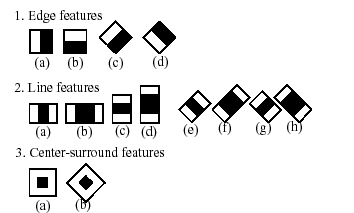
\includegraphics[scale=0.5]{images/haarfeatures.png}
  \caption{Features in Cascade Classifier \cite{haar-opencv-doc}}
  \label{fig:haar-feats}
\end{figure}

For the implementation of the feature extraction and classification we used a library called "facerec"\cite{facerec-lib}.
This provided support for Fisherfaces, Eigenfaces and Local Binary Pattern Histogram as Feature Extraction algorithms and k-Nearest Neighbours and Support Vector Machines as classifiers.

We scripted the program in such a way, that it automatically trains different combinations of the above and provide csv-tables and graphs for the results of the evaluation.

\section{Evaluation of the results}

In figure \ref{fig:acc} the average of the accuracy over the different users is shown against the different feature extraction algorithms and classifiers.
Additionally it differentiates between majority decision (see above) and decision on pictures alone, marked with "\_vote" and "\_nonvote".

As shown in the picture, we got the best combination for all users using PCA (Eigenfaces) as a feature extraction and 5-nearest neighbours with euclidean distance as a classifier.

Assuming random guessing of the algorithm would create an accuracy of 50\%, the graphs show that at least some combinations are significantly better than random, even having the small dataset we tested on in mind.

Shown in the next figures \ref{fig:eigen-acc}, \ref{fig:fish-acc}, \ref{fig:ide-acc} and \ref{fig:spa-acc}, the accuracy of a certain feature is drawn for different classifiers for some selected users.
We assume that these users are representative of the range of errors we got.
The figures clearly state out that the accuracy is highly dependent on the user.
In some cases, like for the user "BabyMonkey", the results of the prediction are even worse then randomly guessing if we assume a rate of 50\%.
In other cases, like for user "mylovelyml", the accuracy is up to over 90\% and shows that the algorithm is capable to select the matching pictures with relatively high accuracy.

The graphs state further, that Fisherface is the worst feature extraction algorithms of the competitors and 5-Nearest Neighbours with Euclidean distance has in general quite high accuracy compared to the competitors.

Nevertheless, we have problems explaining the special behaviour of Fisherface for user "GoTobias" and "mylovelyml".

\begin{figure}[!htb]
  \centering
  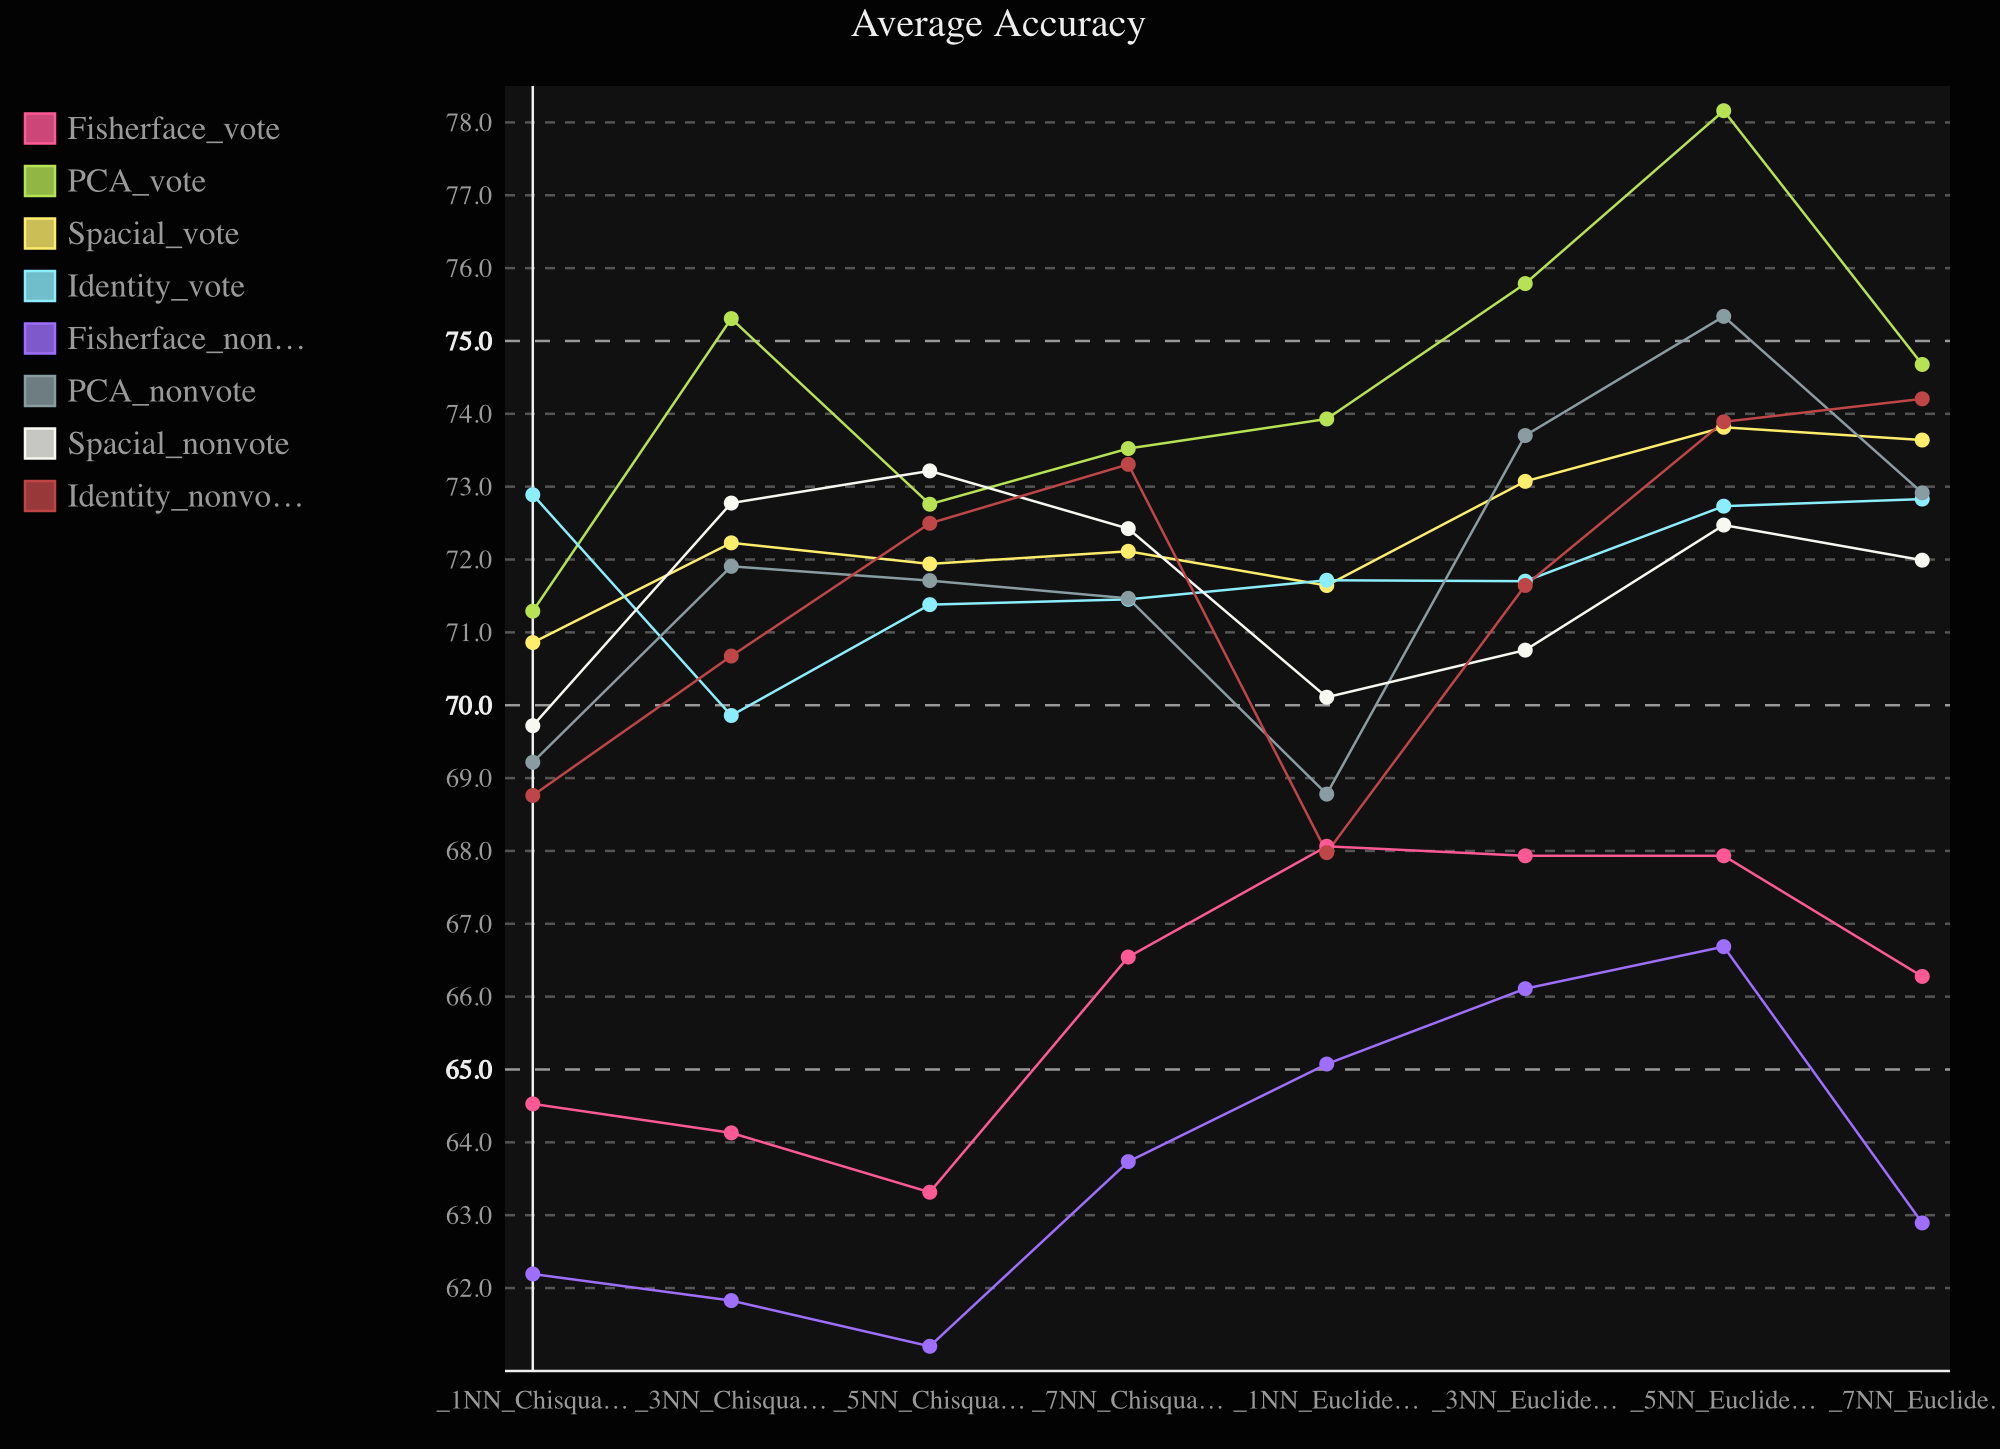
\includegraphics[scale=0.2]{images/accuracy_line.png}
  \caption{Average Accuracy}
  \label{fig:acc}
\end{figure}

\begin{figure}[!htb]
  \centering
  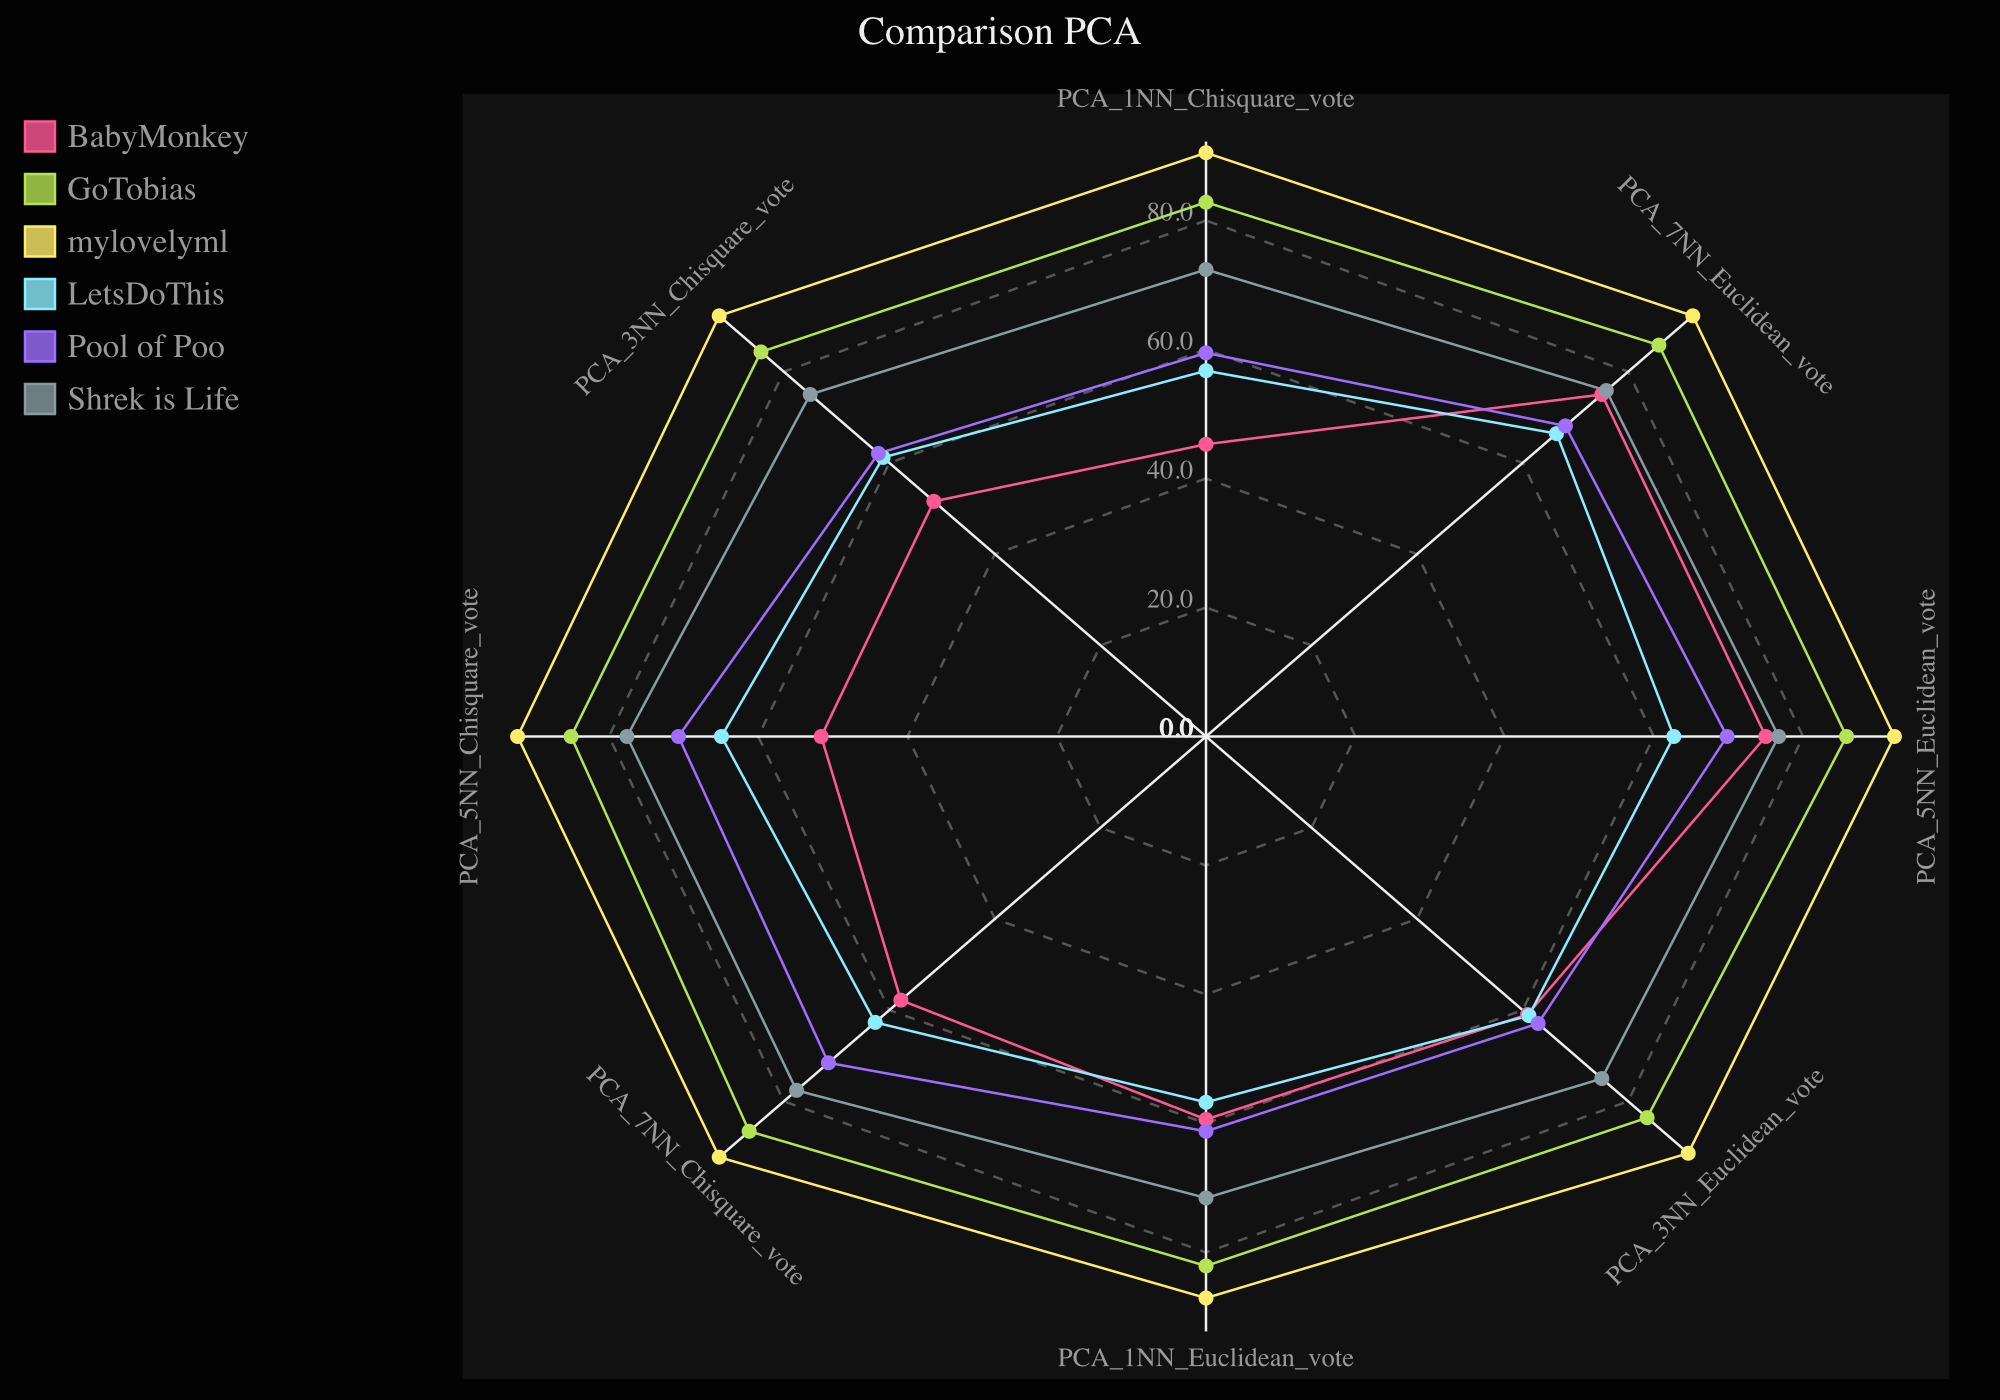
\includegraphics[scale=0.2]{images/PCA_radar.png}
  \caption{Eigenfaces accuracy}
  \label{fig:eigen-acc}
\end{figure}

\begin{figure}[!htb]
  \centering
  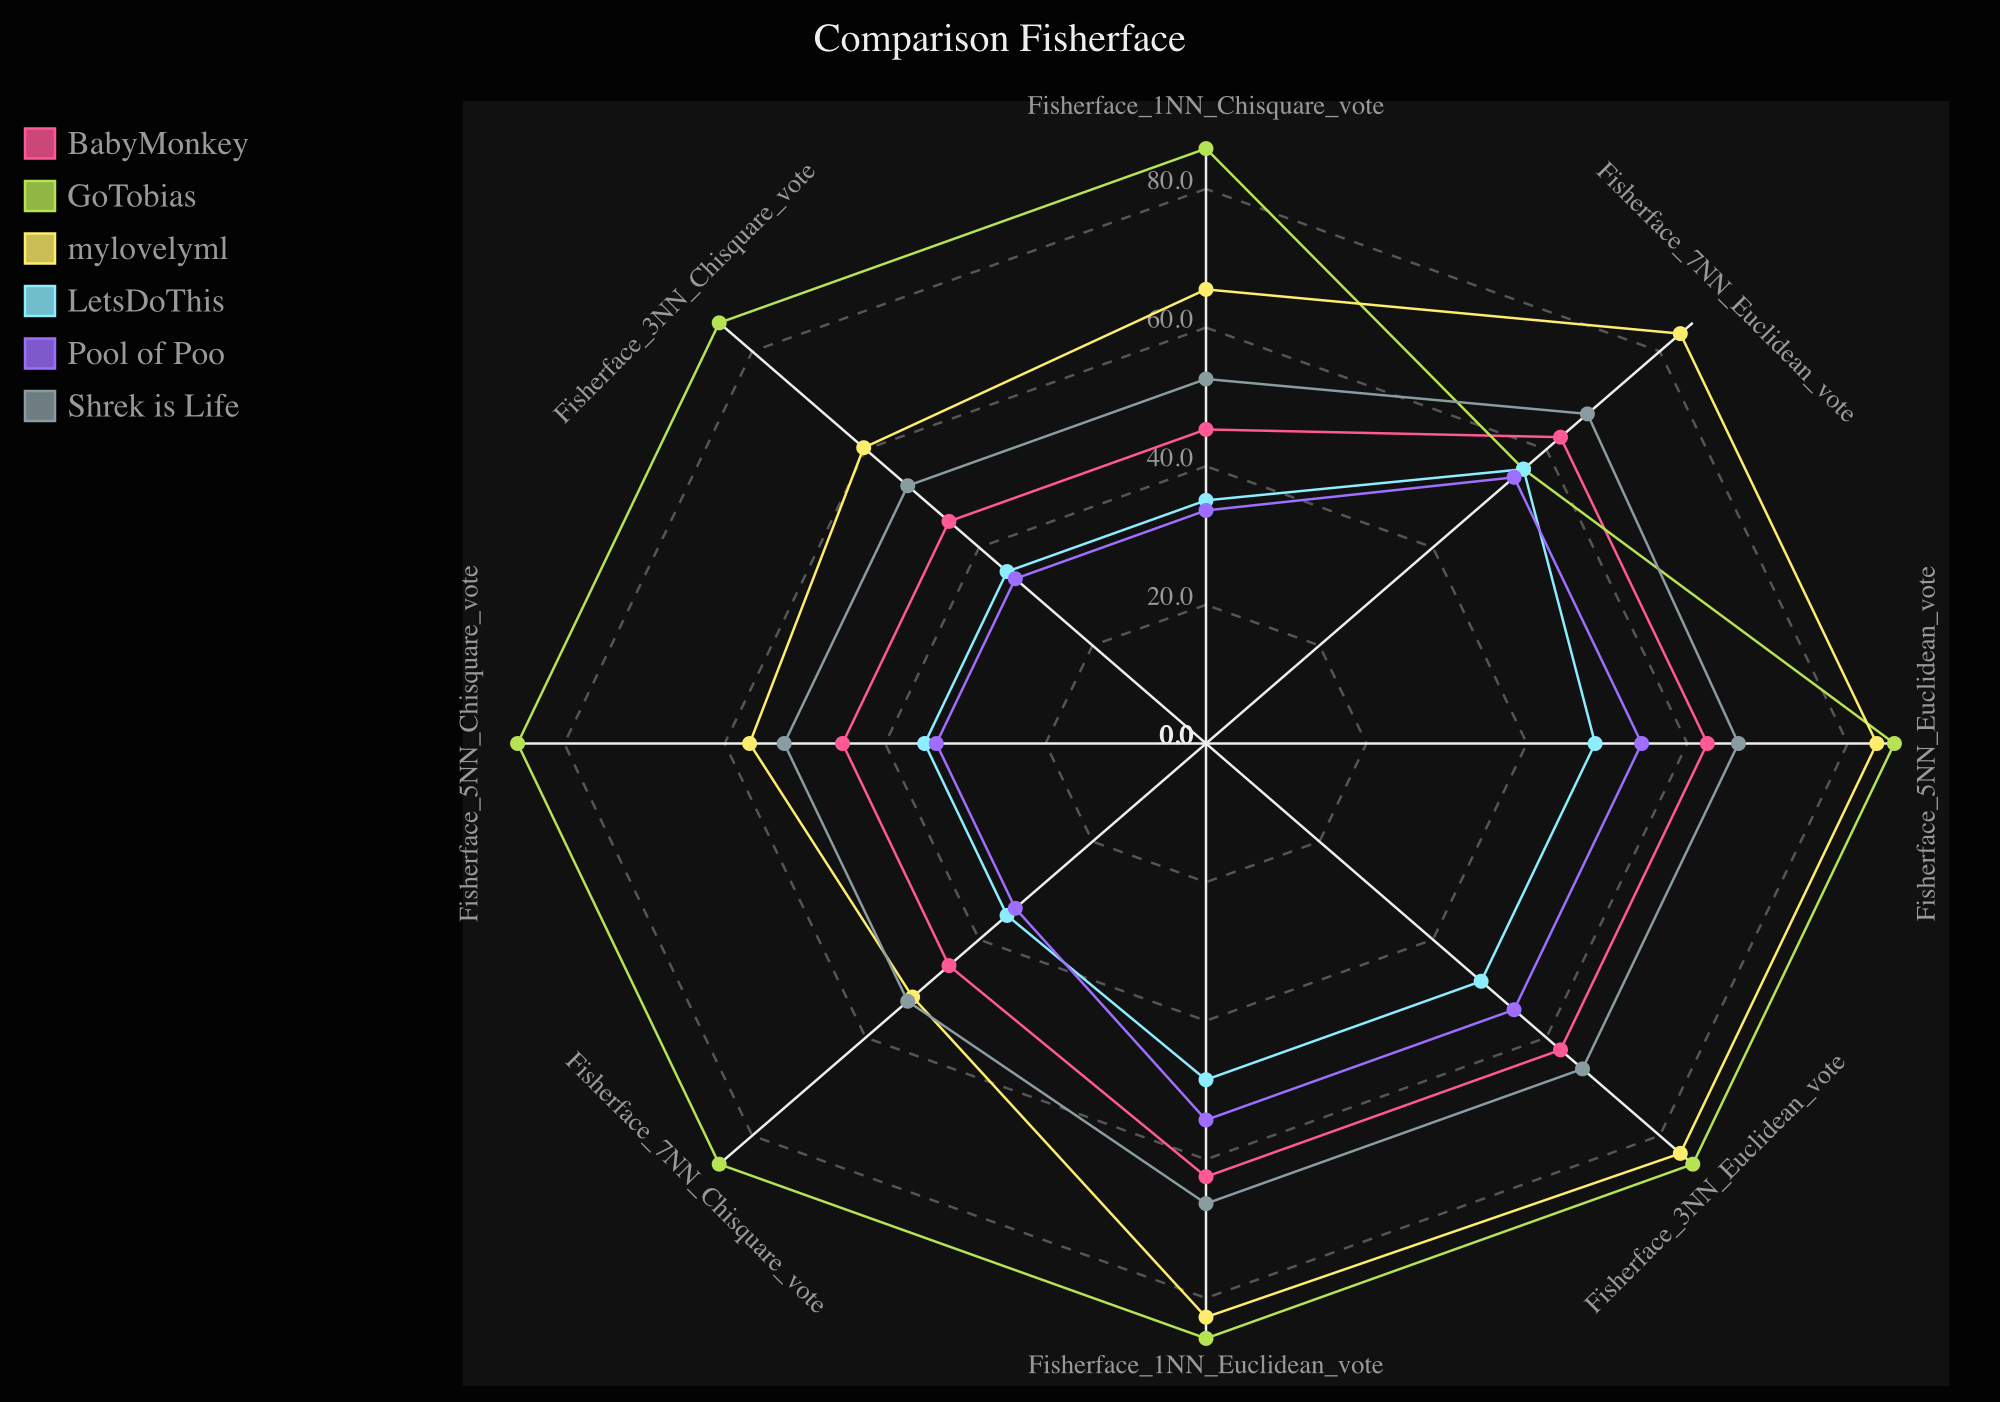
\includegraphics[scale=0.2]{images/Fisherface_radar.png}
  \caption{Fisherfaces accuracy}
  \label{fig:fish-acc}
\end{figure}

\begin{figure}[!htb]
  \centering
  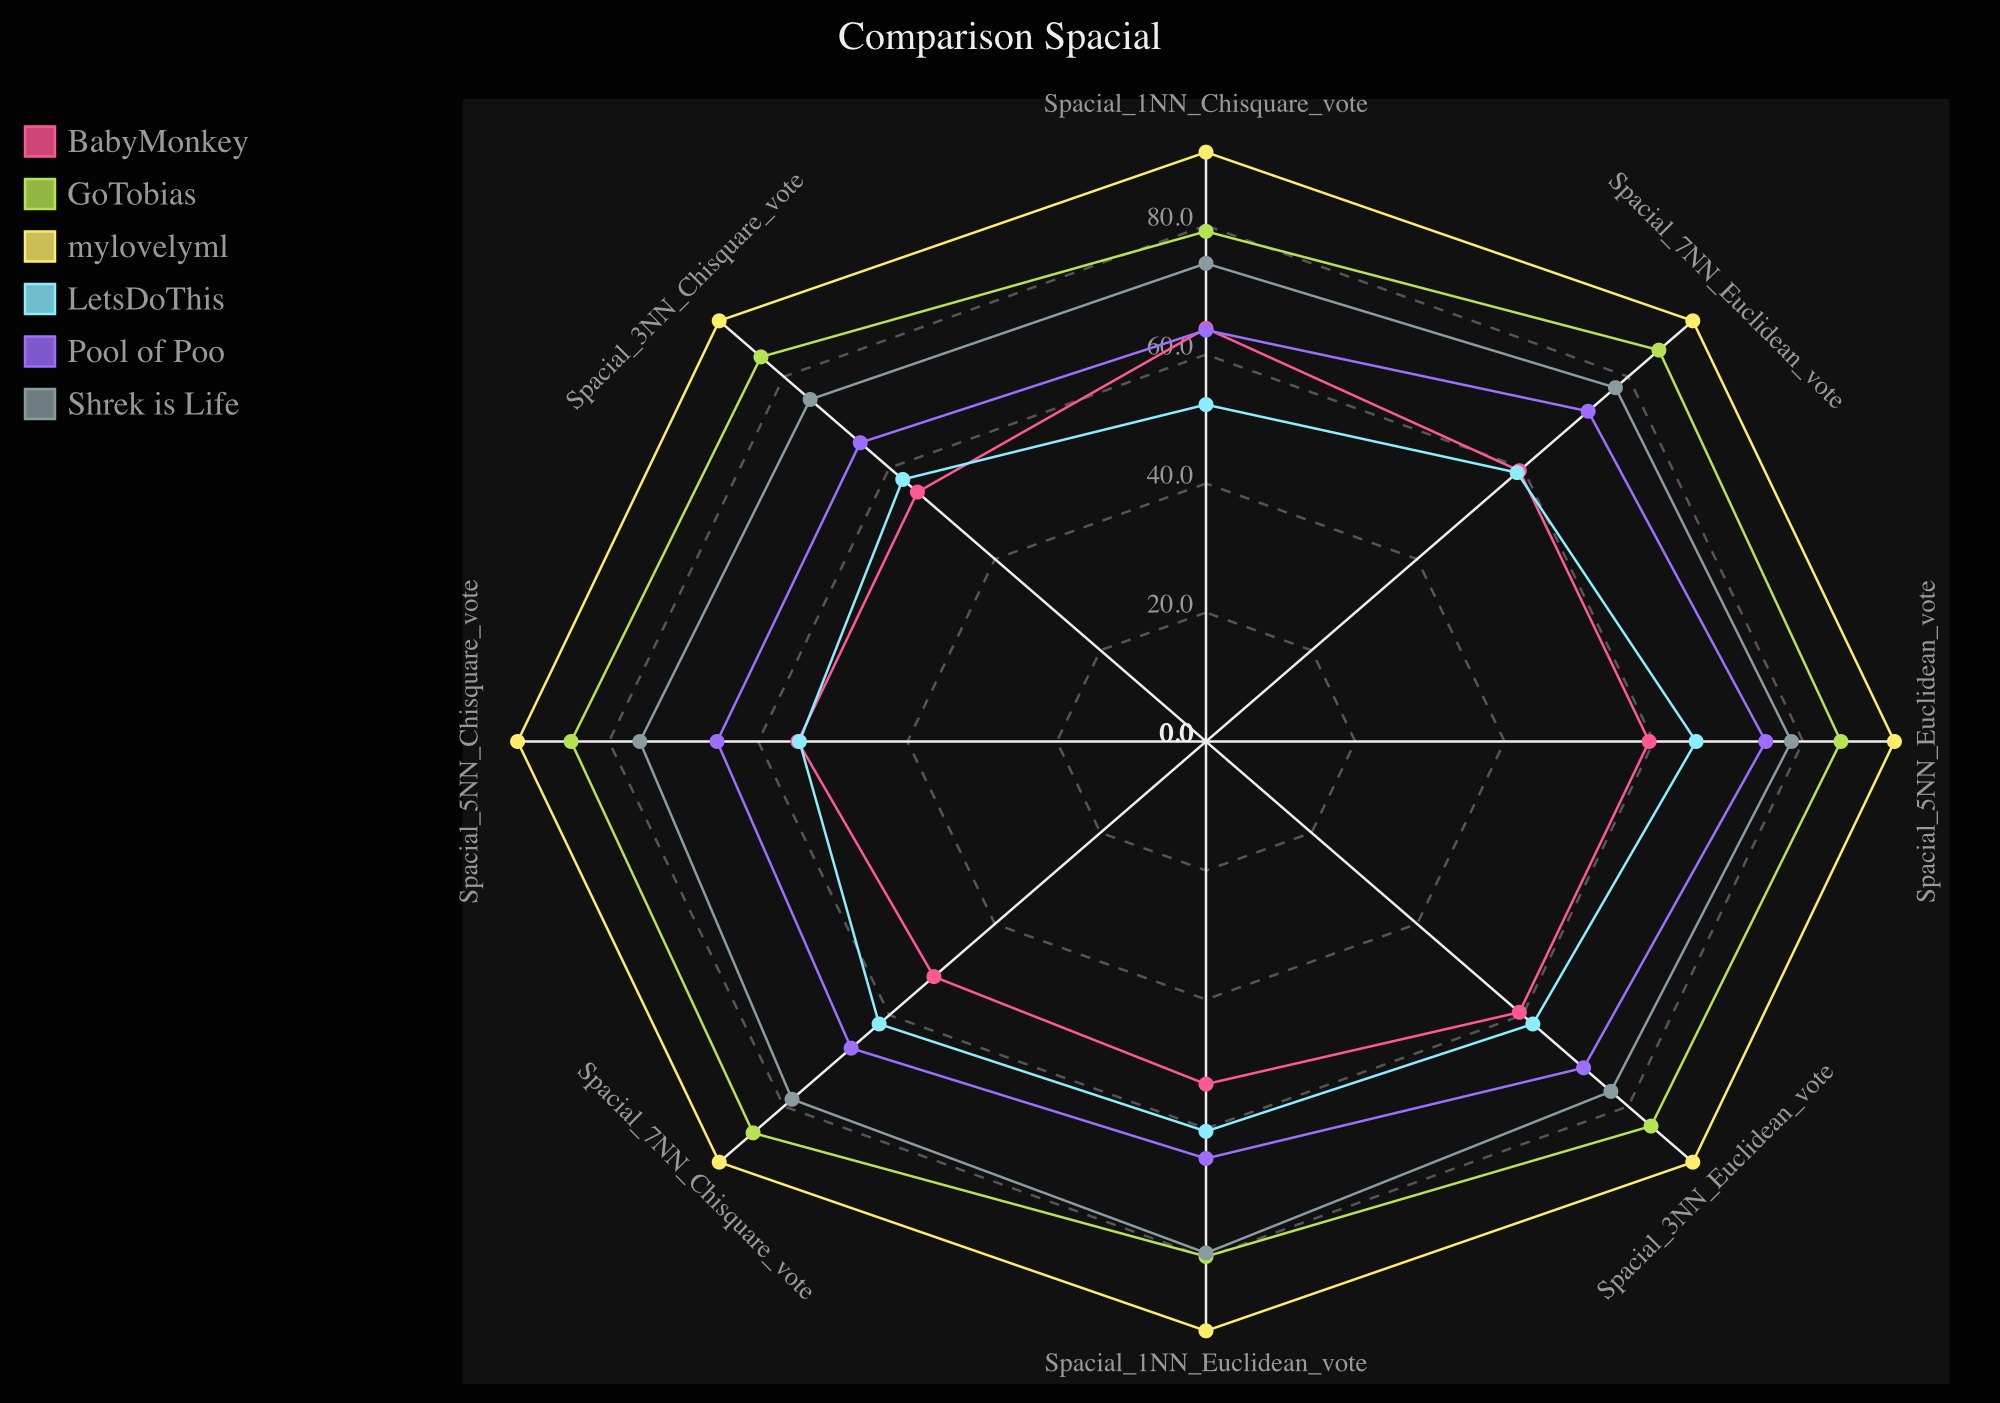
\includegraphics[scale=0.2]{images/Spacial_radar.png}
  \caption{Local Binary Pattern accuracy}
  \label{fig:spa-acc}
\end{figure}

\begin{figure}[!htb]
  \centering
  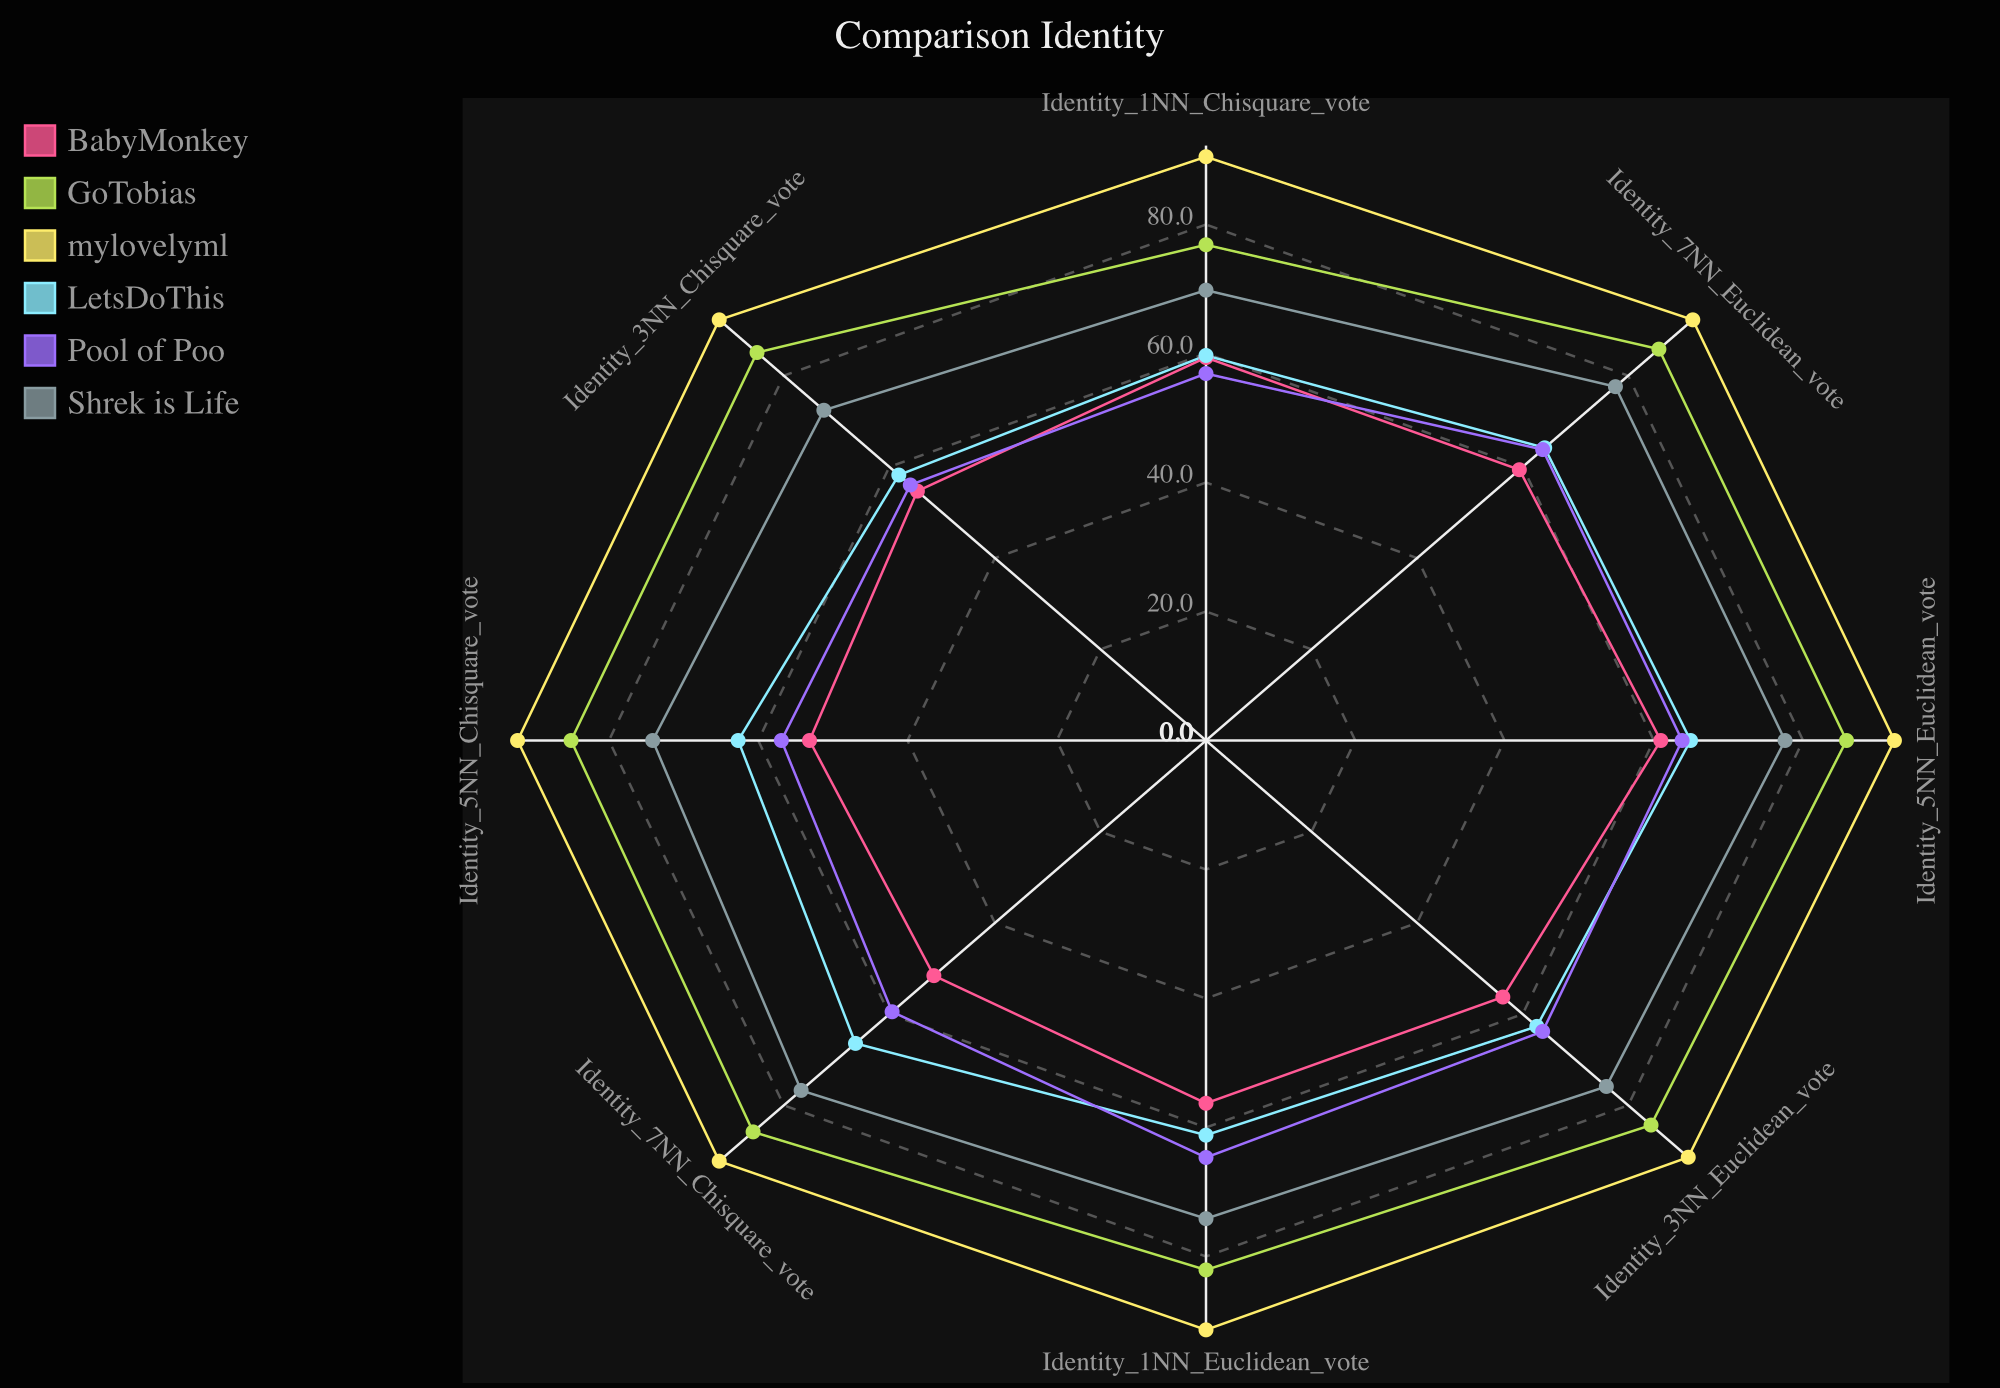
\includegraphics[scale=0.2]{images/Identity_radar.png}
  \caption{Identity accuracy}
  \label{fig:ide-acc}
\end{figure}

\section{Guessing and Significance}
To interpret whether the algorithms work successfully, we have to assume a certain probability for successful random guessing to which we can compare our results.

Assuming the user liked a person with a possibility of 50\%, we should statistically be able to get an accuracy of 50\% using random guessing.
The same holds if a person just likes 10\% and dislikes 90\% of the people.
Nevertheless, in the last case it would be possible to just dislike all persons and get an accuracy of 90\% which would be on the line with our best results.

Concerning that, it is not quite possible for us to state whether the algorithms are better than \emph{educated guessing} or not.

As shown in figure \ref{fig:bargraph-pca} the testcases create false positive as well as false negative results.
The graphs for other combinations of feature extraction and distance functions are comparable.
Because of this behaviour, we assume that 50\% as an error rate for random guessing can be used and the provided graphs show, that at least some combinations are working significantly better then guessing.

\begin{figure}[!htb]
  \centering
  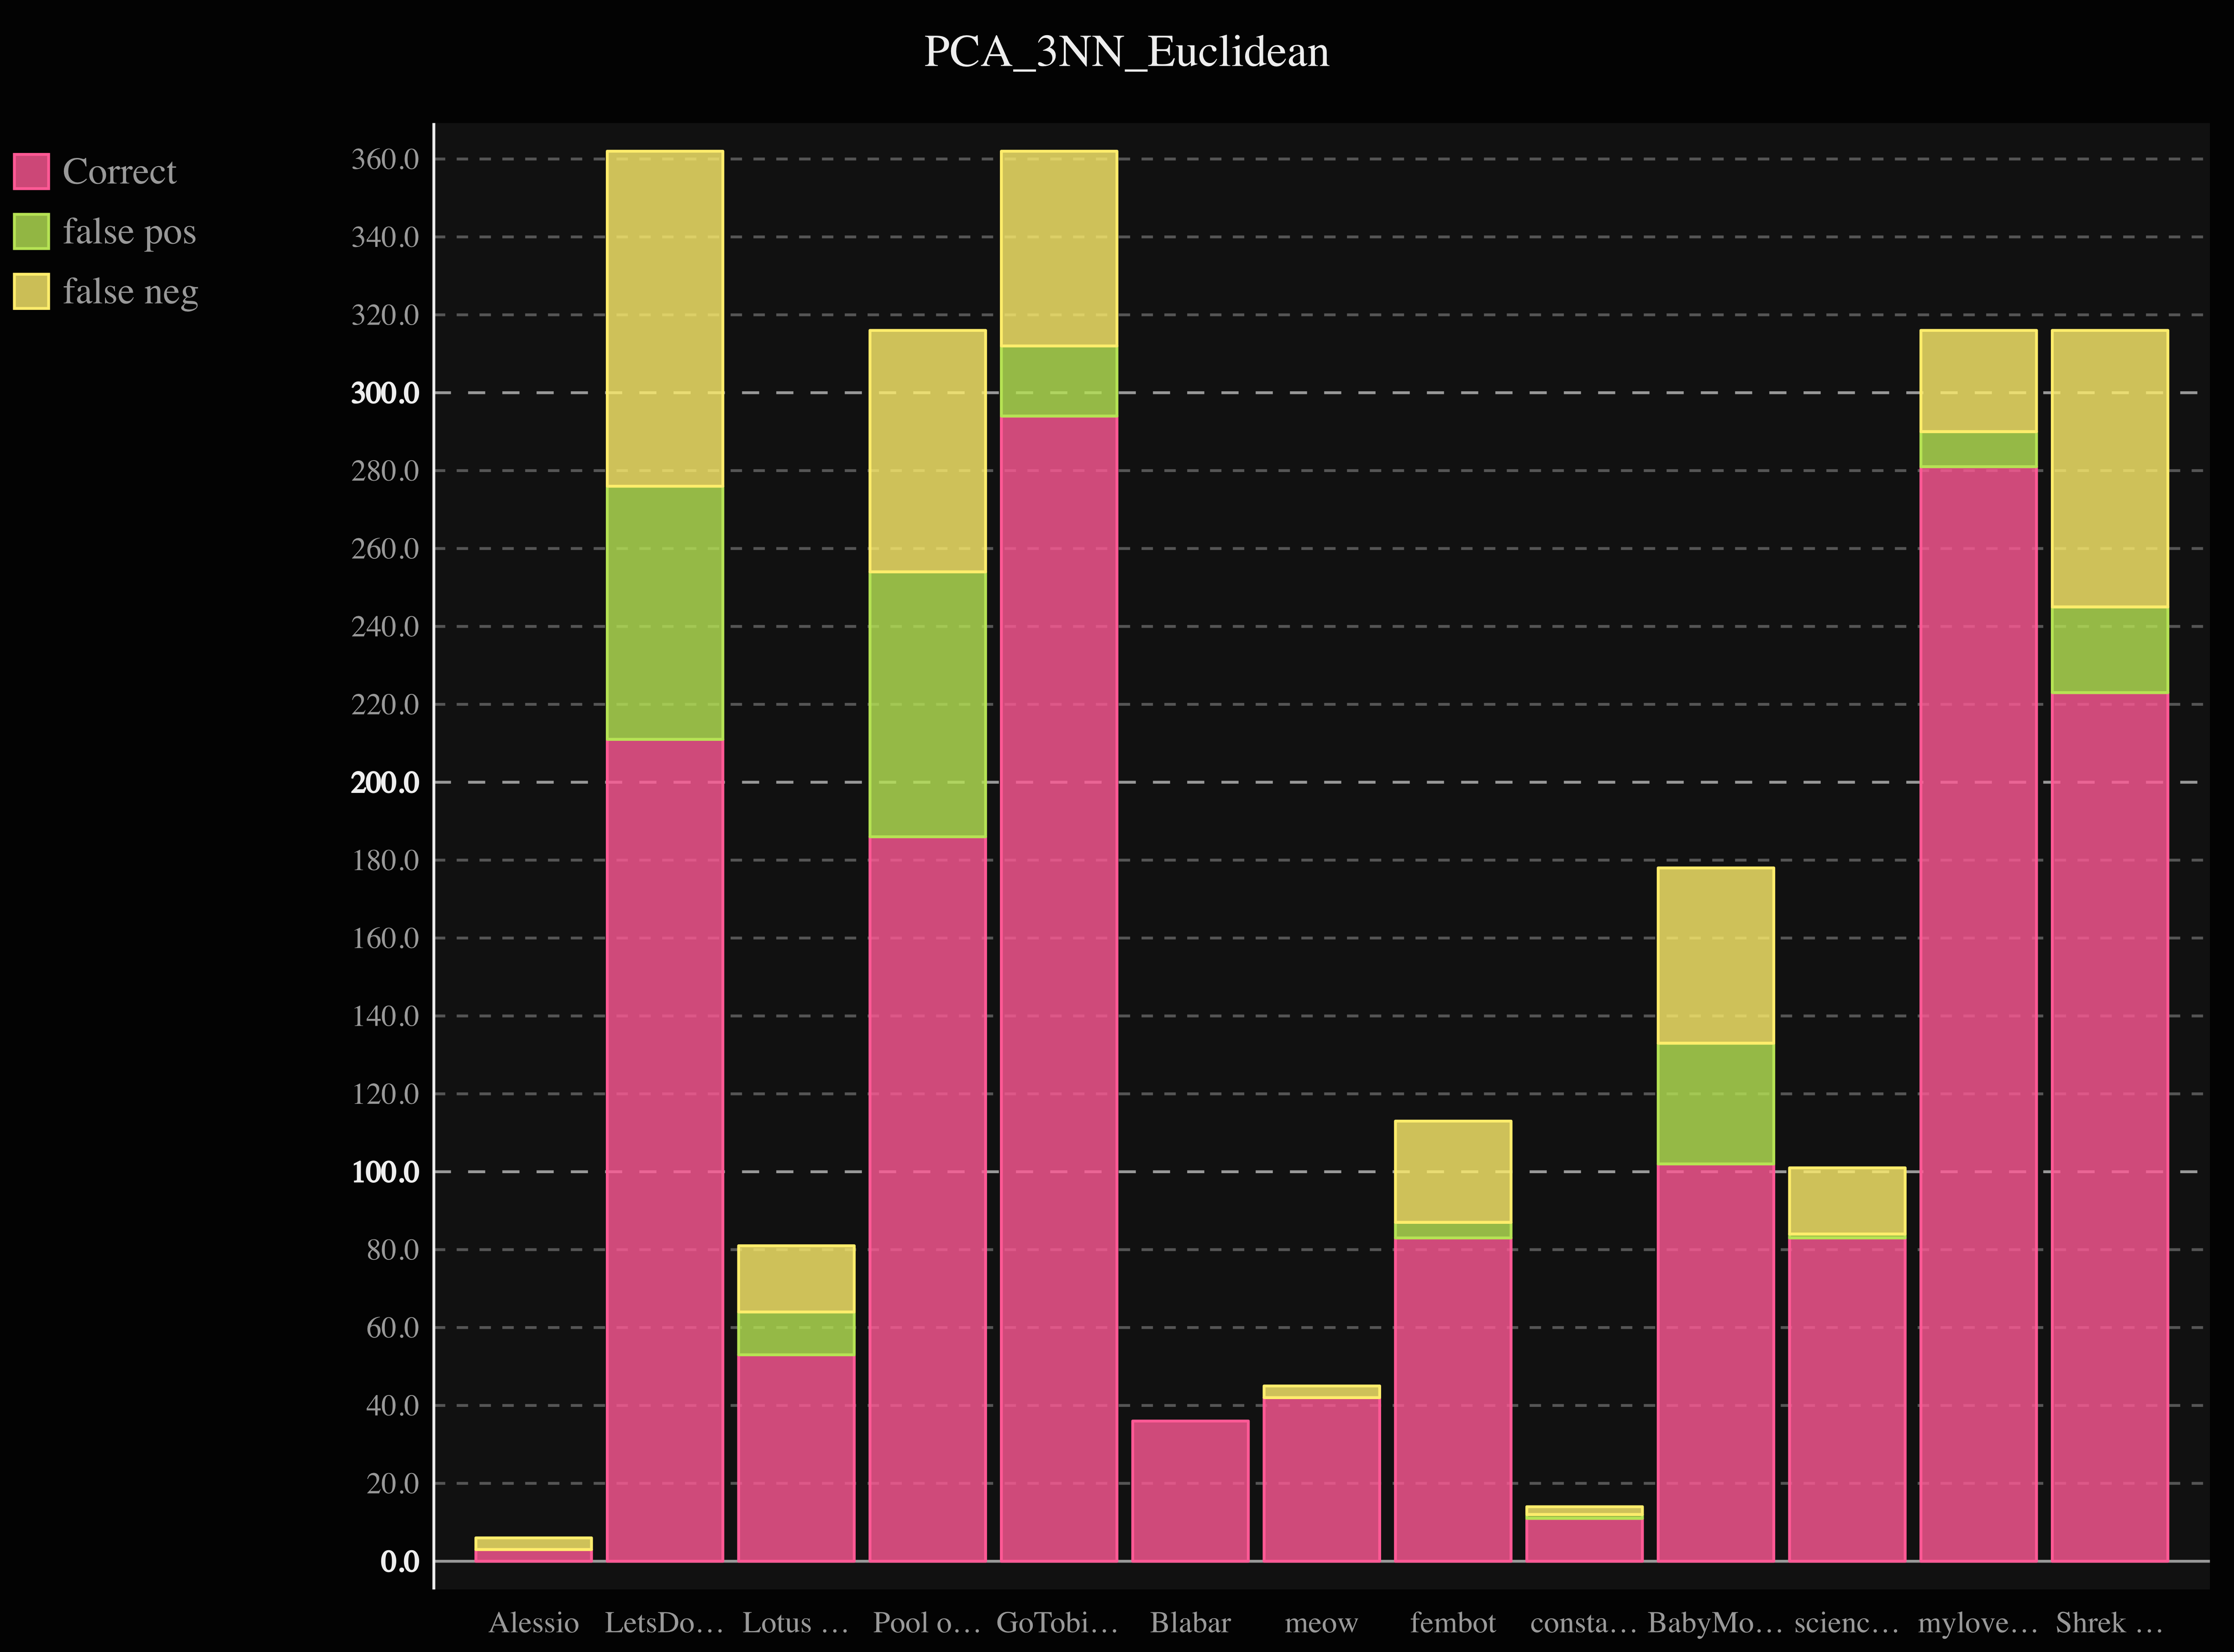
\includegraphics[scale=0.08]{images/PCA_3NN_Euclidean_nonvote.png}
  \caption{accuracy PCA 3NN Euclidean}
  \label{fig:bargraph-pca}
\end{figure}

\clearpage

\subsection{Conclusion}
We know from some persons of the test group, that they had quite some problems to just rate the face that was acutally used by the algorithm and not the person as a whole, including clothes and appearance.
Furthermore, by looking at the cropped images, we found some pictures, where the wrong person was cropped out or the picture was slightly turned.

Concerning these drawbacks in preprocessing and data gathering, we assume, that the data at least for some of the users are quite promising and a basis for further research.

\section{Evaluation of the project}
Overall we think we made a good progress during the project and have some results, which can be used for further investigation.

Nevertheless we had some struggles during the project concerning different versions of Python, support of libraries and the libraries themselves.
The part of gathering the data took a little bit longer then expected and left us less time for optimisation.
Additionally we wanted to also evaluate the use of Support Vector Machines as a classifier and tested the algorithm with different parameters, the results we got back from the library were invalid for all parameters and we were not yet able to fully investigate the error.
Because the algorithm is not just implemented in the library itself but uses also a the bigger libsvm library this might be an encounter which takes us some time, we don't have anymore.

We liked the project and think we learned the basics of how face recognition works in general and how the differnt layers including the machine learning part work together.
We see a lot potential for further improvement we descibed in the next chapter.

\chapter{Related and future works}
This project explores just a small part of the available possibilities. The face recognition algorithms we used were easy to use from the programming point of view as well as well tested. Although, we are aware of the fact that nowadays, more accurate and sophisticated methods are available. For instance, Facebook uses \textit{Deep Learning} system to create a 3D representation of a face given a 2D image \cite{taigman2014deepface}, but this goes beyond our knowledge and from a project point of view, this technique would be too to complicated to implement.

As mentioned in the Introduction, \textit{Tinderbox} is a program that autoselect people on Tinder using face recognition. The application exploits Eigenfaces as features extraction and for each person it detects the face from every picture and computes the mean. After the user has trained a model with ca60 people, the program starts selecting people automatically \cite{tinderbox}.

Different improvements can be applied to this project. One of those could be the use of Support Vector Machine as classification method. Despite our efforts to use this algorithm, we were not able to get the best out of it because of lack of time. The number of parameter that can be tuned and kernel functions in SVM is so large that it could be a potential project itself.
Another enhancement could be the use of different cropping sizes for each image. This could potentially improve the features extraction algorithms because they would have a broader area to work on.

As said above, K-means is still in beta and we do not know when it will be released. Although, it could be a potential feature to use in the future.


%%%%%% Bibliography %%%%%%

\bibliographystyle{ieeetr}
\bibliography{bibliography}

\end{document}
